\documentclass{homeworg}
\usepackage{enumitem}
\usepackage{listings}
\usepackage{color} %red, green, blue, yellow, cyan, magenta, black, white
\definecolor{mygreen}{RGB}{28,172,0} % color values Red, Green, Blue
\definecolor{mylilas}{RGB}{170,55,241}

%\usepackage{authblk}
%\title{CSE 5301 - HW02}
%\author[1]{Bardia Mojra}
%\affil[1]{1000766739}
\begin{document}

% --------------- Title -------------------------------------
%\maketitle
\begin{center}
\textbf{EE 5323 - HW03}\\
\end{center}

\noindent
Bardia Mojra\\
1000766739\\
\today\\
HW03 -- Nonlinear System Simulations\\
EE 5323 -- Nonlinear Systems\\
Dr. Lewis


\exercise
\noindent
\textbf{Voltera Predator-Prey System} \\
Consider the Voltera predator-prey system,\\
$$
\dot{x}_1 = - x_1 + x_1 x_2
$$
$$
\dot{x}_2 = x_2 -  x_1 x_2
$$
Find the equilibrium points and their nature.\\

\noindent
\textbf{Answer} \\
State variable is given as:
$$
~\dot{x}_1 = - x_1 + x_1 x_2
~\dot{x}_2 = x_2 -  x_1 x_2
$$

The Voltera predator-prey system has limit cycles therefore the system is
at equilibrium when the population of both predator and prey remain
constant; thus, the derivative should be zero.
To find the equilibrium, I set $\dot{x}_{1}=0$ and $\dot{x}_{2}=0$.
Solve the system for its roots.\\

$$
~\dot{x}_1 = 0 \Rightarrow 0 =  - x_1 + x_1 x_2
~\dot{x}_2 = 0 \Rightarrow 0 = x_2 -  x_1 x_2
$$
$$
~0 = x_1 (\beta x_2 - \alpha)~\Rightarrow~x_1 = 0 ; ~x_2 = \alpha/\beta
$$
$$~0 = x_2 (\gamma - \sigma x_1)~\Rightarrow~x_1 = \gamma/\sigma ; ~x_2 = 0
$$

There are two equilibrium points at $(x_1,~x_2)$,

\begin{itemize}
  \item At zero, $~(0 ,~ 0),$
  \item Any positive pair of integers $(\alpha/\beta,~\gamma/\sigma)$
\end{itemize}

The equilibrium point nature of the zero is a stable center point that is a
limit cycle. The other e.p. has a saddle point nature because it is stable
in one dimension (goes to zero) and unstable in the other (goes to
infinity).

\lstset{language=Matlab,%
    %basicstyle=\color{red},
    breaklines=true,%
    morekeywords={matlab2tikz},
    keywordstyle=\color{blue},%
    morekeywords=[2]{1}, keywordstyle=[2]{\color{black}},
    identifierstyle=\color{black},%
    stringstyle=\color{mylilas},
    commentstyle=\color{mygreen},%
    showstringspaces=false,%without this there will be a symbol in the places where there is a space
    numbers=left,%
    numberstyle={\tiny \color{black}},% size of the numbers
    numbersep=9pt, % this defines how far the numbers are from the text
    emph=[1]{for,end,break},emphstyle=[1]\color{red}, %some words to emphasise
    %emph=[2]{word1,word2}, emphstyle=[2]{style},
}
\newpage
\noindent
\textbf{Matlab Code}\\
\lstinputlisting{main_HW03_Q01_BM.m}
\newline
\newpage
\noindent
\textbf{Figures}\\
\begin{figure}[h]
  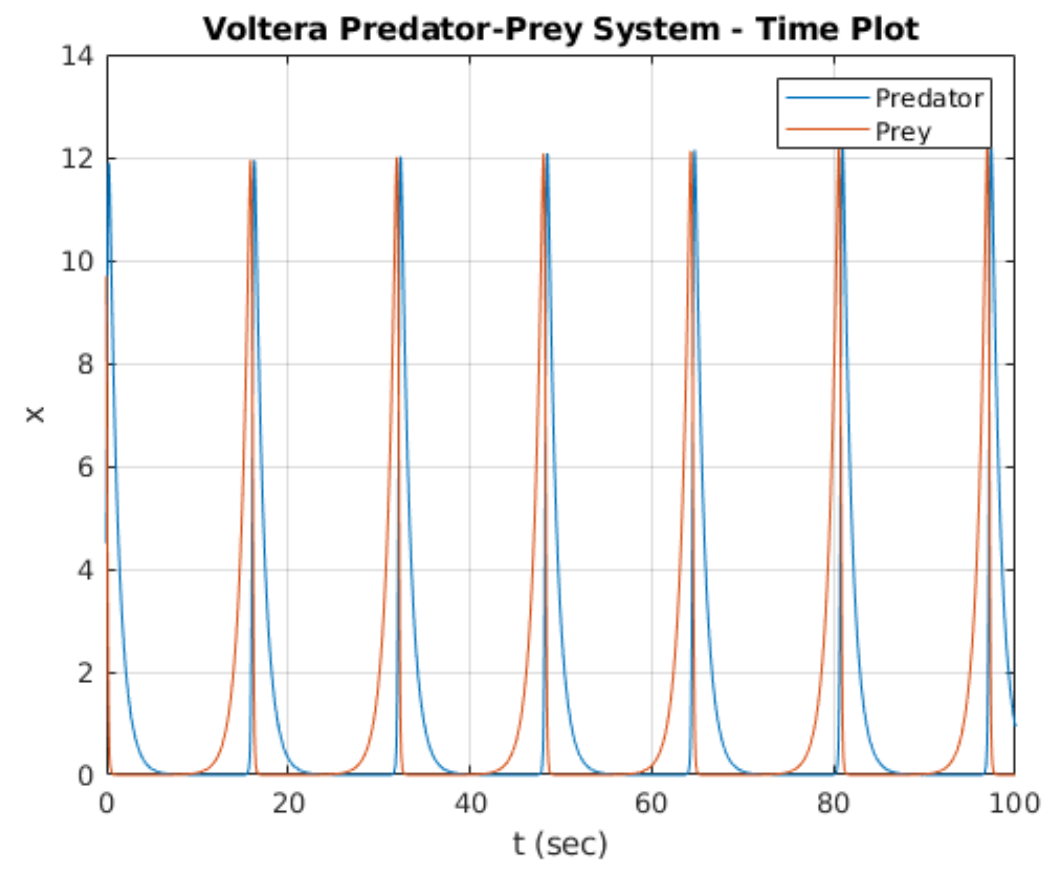
\includegraphics[width=.6\textwidth]{fig001.png}
  \centering
\end{figure}
\begin{figure}[h]
  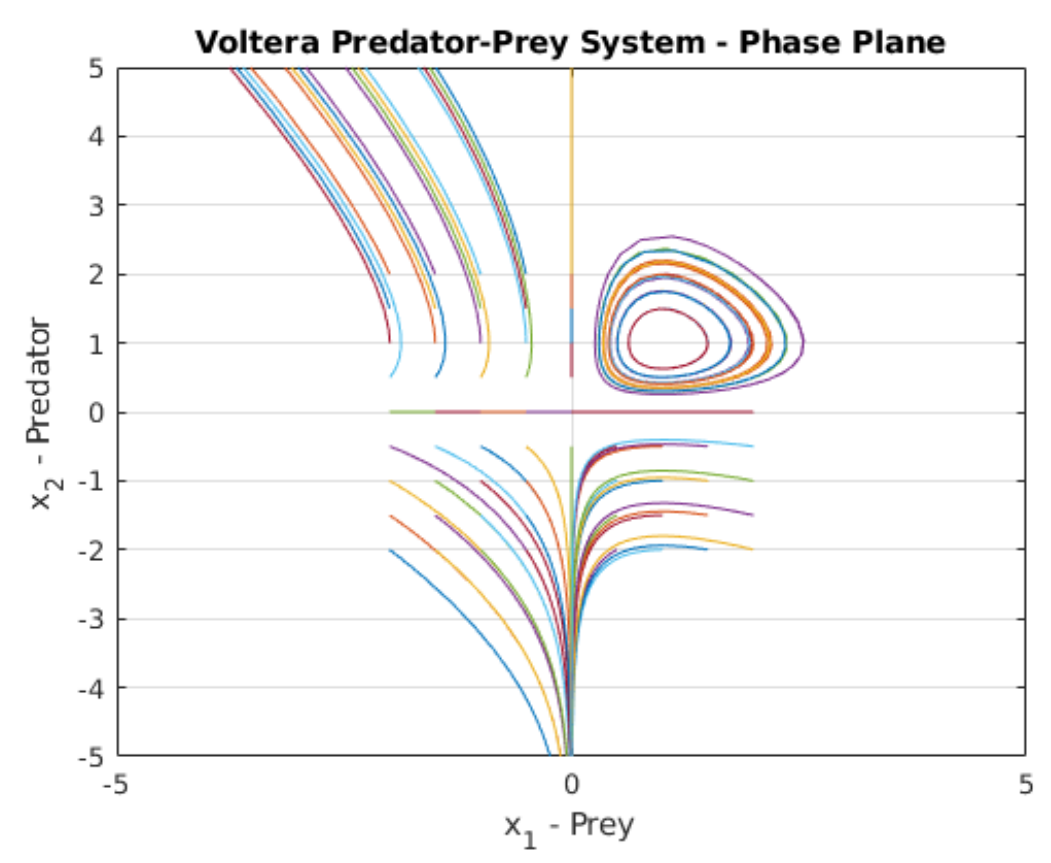
\includegraphics[width=.6\textwidth]{fig002.png}
  \centering
\end{figure}

\exercise
\noindent
\textbf{Equilibrium points and linearization} \\
Consider the following system,\\
$$
\dot{x}_1 = x_2 (- x_1 + x_2 - 1)
$$
$$
\dot{x}_2 = x_1 (x_1 + x_2 + 1)
$$


\begin{enumerate}[label=(\alph*)]
\item Find all equilibrium points
\item Find Jacobian
\item Find the nature of all e.p.s
\end{enumerate}



\noindent
\textbf{Answer} \\
State


%\bibliography{ref}

\end{document}
